% Options for packages loaded elsewhere
\PassOptionsToPackage{unicode}{hyperref}
\PassOptionsToPackage{hyphens}{url}
%
\documentclass[
  11pt,
  letterpaper,
  DIV=11,
  numbers=noendperiod,
  twoside]{scrartcl}

\usepackage{amsmath,amssymb}
\usepackage{setspace}
\usepackage{iftex}
\ifPDFTeX
  \usepackage[T1]{fontenc}
  \usepackage[utf8]{inputenc}
  \usepackage{textcomp} % provide euro and other symbols
\else % if luatex or xetex
  \usepackage{unicode-math}
  \defaultfontfeatures{Scale=MatchLowercase}
  \defaultfontfeatures[\rmfamily]{Ligatures=TeX,Scale=1}
\fi
\usepackage{lmodern}
\ifPDFTeX\else  
    % xetex/luatex font selection
    \setmainfont[ItalicFont=EB Garamond Italic,BoldFont=EB Garamond
Bold]{EB Garamond Math}
    \setsansfont[]{EB Garamond}
  \setmathfont[]{Garamond-Math}
\fi
% Use upquote if available, for straight quotes in verbatim environments
\IfFileExists{upquote.sty}{\usepackage{upquote}}{}
\IfFileExists{microtype.sty}{% use microtype if available
  \usepackage[]{microtype}
  \UseMicrotypeSet[protrusion]{basicmath} % disable protrusion for tt fonts
}{}
\usepackage{xcolor}
\usepackage[left=1.1in, right=1in, top=0.8in, bottom=0.8in,
paperheight=9.5in, paperwidth=7in, includemp=TRUE, marginparwidth=0in,
marginparsep=0in]{geometry}
\setlength{\emergencystretch}{3em} % prevent overfull lines
\setcounter{secnumdepth}{3}
% Make \paragraph and \subparagraph free-standing
\makeatletter
\ifx\paragraph\undefined\else
  \let\oldparagraph\paragraph
  \renewcommand{\paragraph}{
    \@ifstar
      \xxxParagraphStar
      \xxxParagraphNoStar
  }
  \newcommand{\xxxParagraphStar}[1]{\oldparagraph*{#1}\mbox{}}
  \newcommand{\xxxParagraphNoStar}[1]{\oldparagraph{#1}\mbox{}}
\fi
\ifx\subparagraph\undefined\else
  \let\oldsubparagraph\subparagraph
  \renewcommand{\subparagraph}{
    \@ifstar
      \xxxSubParagraphStar
      \xxxSubParagraphNoStar
  }
  \newcommand{\xxxSubParagraphStar}[1]{\oldsubparagraph*{#1}\mbox{}}
  \newcommand{\xxxSubParagraphNoStar}[1]{\oldsubparagraph{#1}\mbox{}}
\fi
\makeatother


\providecommand{\tightlist}{%
  \setlength{\itemsep}{0pt}\setlength{\parskip}{0pt}}\usepackage{longtable,booktabs,array}
\usepackage{calc} % for calculating minipage widths
% Correct order of tables after \paragraph or \subparagraph
\usepackage{etoolbox}
\makeatletter
\patchcmd\longtable{\par}{\if@noskipsec\mbox{}\fi\par}{}{}
\makeatother
% Allow footnotes in longtable head/foot
\IfFileExists{footnotehyper.sty}{\usepackage{footnotehyper}}{\usepackage{footnote}}
\makesavenoteenv{longtable}
\usepackage{graphicx}
\makeatletter
\newsavebox\pandoc@box
\newcommand*\pandocbounded[1]{% scales image to fit in text height/width
  \sbox\pandoc@box{#1}%
  \Gscale@div\@tempa{\textheight}{\dimexpr\ht\pandoc@box+\dp\pandoc@box\relax}%
  \Gscale@div\@tempb{\linewidth}{\wd\pandoc@box}%
  \ifdim\@tempb\p@<\@tempa\p@\let\@tempa\@tempb\fi% select the smaller of both
  \ifdim\@tempa\p@<\p@\scalebox{\@tempa}{\usebox\pandoc@box}%
  \else\usebox{\pandoc@box}%
  \fi%
}
% Set default figure placement to htbp
\def\fps@figure{htbp}
\makeatother
% definitions for citeproc citations
\NewDocumentCommand\citeproctext{}{}
\NewDocumentCommand\citeproc{mm}{%
  \begingroup\def\citeproctext{#2}\cite{#1}\endgroup}
\makeatletter
 % allow citations to break across lines
 \let\@cite@ofmt\@firstofone
 % avoid brackets around text for \cite:
 \def\@biblabel#1{}
 \def\@cite#1#2{{#1\if@tempswa , #2\fi}}
\makeatother
\newlength{\cslhangindent}
\setlength{\cslhangindent}{1.5em}
\newlength{\csllabelwidth}
\setlength{\csllabelwidth}{3em}
\newenvironment{CSLReferences}[2] % #1 hanging-indent, #2 entry-spacing
 {\begin{list}{}{%
  \setlength{\itemindent}{0pt}
  \setlength{\leftmargin}{0pt}
  \setlength{\parsep}{0pt}
  % turn on hanging indent if param 1 is 1
  \ifodd #1
   \setlength{\leftmargin}{\cslhangindent}
   \setlength{\itemindent}{-1\cslhangindent}
  \fi
  % set entry spacing
  \setlength{\itemsep}{#2\baselineskip}}}
 {\end{list}}
\usepackage{calc}
\newcommand{\CSLBlock}[1]{\hfill\break\parbox[t]{\linewidth}{\strut\ignorespaces#1\strut}}
\newcommand{\CSLLeftMargin}[1]{\parbox[t]{\csllabelwidth}{\strut#1\strut}}
\newcommand{\CSLRightInline}[1]{\parbox[t]{\linewidth - \csllabelwidth}{\strut#1\strut}}
\newcommand{\CSLIndent}[1]{\hspace{\cslhangindent}#1}

\setlength\heavyrulewidth{0ex}
\setlength\lightrulewidth{0ex}
\usepackage[automark]{scrlayer-scrpage}
\clearpairofpagestyles
\cehead{
  Brian Weatherson
  }
\cohead{
  Why Do Decision Theory?
  }
\ohead{\bfseries \pagemark}
\cfoot{}
\makeatletter
\newcommand*\NoIndentAfterEnv[1]{%
  \AfterEndEnvironment{#1}{\par\@afterindentfalse\@afterheading}}
\makeatother
\NoIndentAfterEnv{itemize}
\NoIndentAfterEnv{enumerate}
\NoIndentAfterEnv{description}
\NoIndentAfterEnv{quote}
\NoIndentAfterEnv{equation}
\NoIndentAfterEnv{longtable}
\NoIndentAfterEnv{abstract}
\renewenvironment{abstract}
 {\vspace{-1.25cm}
 \quotation\small\noindent\emph{Abstract}:}
 {\endquotation}
\newfontfamily\tfont{EB Garamond}
\addtokomafont{disposition}{\rmfamily}
\addtokomafont{title}{\normalfont\itshape}
\let\footnoterule\relax
\KOMAoption{captions}{tableheading}
\makeatletter
\@ifpackageloaded{caption}{}{\usepackage{caption}}
\AtBeginDocument{%
\ifdefined\contentsname
  \renewcommand*\contentsname{Table of contents}
\else
  \newcommand\contentsname{Table of contents}
\fi
\ifdefined\listfigurename
  \renewcommand*\listfigurename{List of Figures}
\else
  \newcommand\listfigurename{List of Figures}
\fi
\ifdefined\listtablename
  \renewcommand*\listtablename{List of Tables}
\else
  \newcommand\listtablename{List of Tables}
\fi
\ifdefined\figurename
  \renewcommand*\figurename{Figure}
\else
  \newcommand\figurename{Figure}
\fi
\ifdefined\tablename
  \renewcommand*\tablename{Table}
\else
  \newcommand\tablename{Table}
\fi
}
\@ifpackageloaded{float}{}{\usepackage{float}}
\floatstyle{ruled}
\@ifundefined{c@chapter}{\newfloat{codelisting}{h}{lop}}{\newfloat{codelisting}{h}{lop}[chapter]}
\floatname{codelisting}{Listing}
\newcommand*\listoflistings{\listof{codelisting}{List of Listings}}
\makeatother
\makeatletter
\makeatother
\makeatletter
\@ifpackageloaded{caption}{}{\usepackage{caption}}
\@ifpackageloaded{subcaption}{}{\usepackage{subcaption}}
\makeatother

\usepackage{bookmark}

\IfFileExists{xurl.sty}{\usepackage{xurl}}{} % add URL line breaks if available
\urlstyle{same} % disable monospaced font for URLs
\hypersetup{
  pdftitle={Why Do Decision Theory?},
  pdfauthor={Brian Weatherson},
  hidelinks,
  pdfcreator={LaTeX via pandoc}}


\title{Why Do Decision Theory?}
\author{Brian Weatherson}
\date{2025}

\begin{document}
\maketitle
\begin{abstract}
What question are decision theorists trying to answer, and why is it
worth trying to answer it? A lot of philosophers talk as if the aim of
decision theory is articulate a standard for making decisions well, and
the reason to do this is to help us make better decisions. I disagree on
both fronts. The aim of the decision theory is, or at least should be,
to describe how a certain kind of idealised decider does in fact decide.
The reason to do this is that this idealisation, like many other
idealisations, helps generate explanations of real-world behaviour. We
shouldn't do what these ideal deciders do, or try to be more like them,
because a lot of what they do only makes sense because of the
differences between us and them. Still, sometimes those differences are
small enough that they can be ignored in explanations, and that's when
decision theory is useful.
\end{abstract}


\setstretch{1.1}
\section{Introduction}\label{sec-intro}

What are we doing when we do decision theory? What questions are
decision theorists trying to answer? And what do we gain by knowing
those answers?

Most philosophical decision theorists would answer these questions with
something like the view I'll call \textbf{prescriptivism}. We're trying
to say how people should ideally decide, and knowing how people should
decide will help people make better decisions. On this model, the
decision theorist is like a high school coach saying ``Here's how the
good ones make decisions, now go out and act like them.''

I'm going to argue against prescriptivism, and in favour of
\textbf{explanationism}. According to explanationism, decision theory is
primarily a descriptive project. It says this is how people actually
make decisions, at least approximately, some of the time. What we gain
from this is access to a certain kind of explanation of various social
phenomena. On this model, the decision theorist is like a high school
science teacher saying ``Here's how things work in a very simplified
model, but even this simplified model shows you something about the
world.''

The big difference between the two views comes in how they treat the
idealisations involved in decision theory. I'll spend some time in this
paper on just what those idealisations are, though hopefully the point
that there are some is common ground. On the prescriptivist view, when
we say that a decision maker ideally does X, we mean that doing X is
perfect, and we should aim to be a more perfect deciders. On the
explanationist view, the idealisations are models.\footnote{Whether they
  are what Weisberg (\citeproc{ref-Weisberg2007}{2007}) calls ``Galilean
  idealisations'' or ``minimal idealisations'' depends on just what use
  they are being put to. The ones that I'm going to talk about are
  primarily the latter.} These models are not standards of perfection.
We don't think the fact that molecules in the toy model used to derive
the ideal gas law are point-sized mean that having zero volume is a
perfection, or that it is better for molecules to be smaller. It's just
that their size is unimportant for the phenomena we're explaining, and
so we abstract away from it.

I'll start with two reasons for rejecting the prescriptivist view. One
is that it does not treat like cases alike. In particular, it makes a
distinction between empirical uncertainty and arithmetic uncertainty
that it should not, were it a prescriptive theory. The second is that it
would be bad to resemble the `ideal' in some respects. To play its
prescriptive role, decision theory would have to be supplemented with a
theory about which aspects of the ideal are and are not worthy of
emulation. There isn't much work on this question, and it isn't at all
clear that it would be easier to solve it than to directly provide
workable advice.

Setting out the objections to prescriptivism is relatively easy.
Defending explanationism is harder going. There are three obvious
objections. The first is that it's a bad description, since people
obviously don't act the way decision theory says they do. This, I think,
is a fairly weak objection and I won't spend much time on it. People do
not act exactly like the theory says, but no model describes exactly how
the subject behaves. As the cliche goes, all models are wrong, but some
models are useful.

This leads to the second objection, which is much more worrying. This
model, says the objector, is not in fact useful. Sure it tells us that
people who prefer vanilla ice cream are more likely to order it. But we
didn't need a whole field of philosophy to tell us that. What are the
interesting explanations the theory offers? Here I follow a suggestion
from Kate Vredenburgh (\citeproc{ref-Vredenburgh2024}{2024}). The
interestiing explanations around here are not individual, but social.
Vredenburgh uses the model of segregation in Schelling
(\citeproc{ref-Schelling1971}{1971}) as her main example.\footnote{This
  is also used as one kind of paradigm model by Weisberg
  (\citeproc{ref-MWeisberg2013}{2013}), so it clearly fits in nicely
  with the picture of decision theory as modeling. A key point that
  Vredenburgh makes is that the kind of functional states that decision
  theory uses are particularly apt for use in explanation here because
  we want to stress what's common to the actors in a model like this,
  even if the functional states are realised differently in different
  actors.}

I'm going to focus on a closely related but distinct class of
explanations, what I'll call \textbf{reflexive explanations}. A
reflexive explanation is one where the fact that agents in the model
believe that the model is correct is partially responsible for the model
working. Most game-theoretic explanations are reflexive in this sense.
The main example I'll use is the model of the used car market that
George Akerlof (\citeproc{ref-Akerlof1970}{1970}) developed, though I'll
also look at some recent work on the software industry. In both cases
I'll argue that decision theory is a vital input into interesting
explanations.

The third objection is that if decision theory earns its keep in the
explanation of empirical regularities, like the surprisingly low price
of used cars, it's odd that it is such an a priori discipline. Here the
fact that it plays a role in explanations that are reflexive will be
crucial. It's only the fact that decision theory is putatively a theory
of rational choice that makes it fit to enter into reflexive
explanations.

{[}Add paragraph about Roussos and other predecessors.{]}

\section{Two Initial Objections}\label{sec-two}

One critic reads the introduction and says that the task I've set is too
easy. I'm asking what we do when we do decision theory, and he says
that's simple. We're trying to say what \emph{rational} choice is. Don't
I know what rationality is, he demands. No, I say, I don't. And I'll say
more in \textbf{?@sec-two-problems} about why I find this so unclear.

Another critic says that the task is too hard. Look at the range of
various theories of decision out there on the market, he says. At this
point he produces a paper where he provides a short summary of the
theories put forward by Lara Buchak (\citeproc{ref-BuchakRisk}{2013}),
Arif Ahmed (\citeproc{ref-Ahmed2014}{2014}), Ben Levinstein and Nate
Soares (\citeproc{ref-LevinsteinSoares2020}{2020}), William Harper
(\citeproc{ref-Harper1986}{1986}), James Joyce
(\citeproc{ref-Joyce1999}{1999}), Frank Arntzenius
(\citeproc{ref-Arntzenius2008}{2008}), Johan Gustafsson
(\citeproc{ref-Gustafsson2011}{2011}), Ralph Wedgwood
(\citeproc{ref-Wedgwood2013a}{2013}), Dmitri Gallow
(\citeproc{ref-Gallow2020}{2020}), Abelard Podgorski
(\citeproc{ref-Podgorski2022}{2022}), David Barnett
(\citeproc{ref-Barnett2022}{2022}), Jack Spencer
(\citeproc{ref-Spencer2023}{2023}) and Melissa Fusco
(\citeproc{ref-Fuscond}{n.d.}). The paper goes on to provide, for each
pair of views, a case where they disagree, along with his verdict about
which theory gets the case right. It's not for the faint of heart. How,
he demands, can I find something in common between those?

There are two replies to such a critic. First, intuitively these
theories disagree. That suggests that there is a common question to
which they are offering competing answers. My job is to find that
question. Second, amidst this flurry of disagreement, there are points
of agreement. I'll focus (also in \textbf{?@sec-two-problems}) on two
cases where they basically all agree. I say `basically' because Buchak
puts forward a family of rivals to orthodox theories, and the views she
calls risk-seeking don't agree with everyone else on one of the cases.
But the risk-averse views, which are her primary focus, do agree with
all the other views listed.

It's going to turn out those two cases alone are enough to raise
problems for prescriptivism, and indeed to make it a bit mysterious what
we could be up to when we do decision theory.

\section{Clarifying the Views}\label{sec-clarify}

Prescriptivism and Explanationism are views about why we do decision
theory. They are views about the reasons for doing decision theory. Like
all questions about reasons, they can be read as questions about
justifying reasons, or about motivating reasons. I'm interested in both,
but this paper is primarily about justifying reasons. There is an
interesting analogy to be drawn between the view that explanationism is
the right theory of motivating reasons and varieties of hermeneutic
fictionalism (\citeproc{ref-Eklund}{\textbf{Eklund?}} §2.2), but I'll
leave that for another day. For now the view is about what is a good
reason to do decision theory, and my argument is that prescriptivism
provides a bad reason, while explanationism provides a good reason.

I've stated these two views fairly informally so far; let's make them
more precise. Both of them are conjunctions of two related but in
principle distinct theses. First prescriptivism, which is \textbf{P1}
and \textbf{P2}:

\begin{description}
\tightlist
\item[P1]
Decision theory describes what ideal deciders are like, and provides a
standard of evaluation for actual deciders: good deciders resemble the
ideal.
\item[P2]
The point of doing decision theory is to provide guidance and advice for
actual deciders. By seeing the ideal more clearly, actual deciders can
improve by coming to resemble it in more respects.
\end{description}

P1 says that the kind of ideal is a standard of perfection, and P2 says
that describing that standard is to provide useful advice. In place of
those, explanationism offers to contrary theses, \textbf{E1} and
\textbf{E2}:

\begin{description}
\tightlist
\item[E1]
Decision theory describes what ideal deciders are like, and predicts
that in suitable circumstances, actual deciders will resemble them.
\item[E2]
The point of doing decision theory is to provide an input into
explanations of social phenomena, in cases where actual deciders behave
sufficiently similarly to ideal deciders.
\end{description}

The ideal is a kind of model, and like all good models, it is a useful
input into good explanations.

There is a third view which is interesting but I won't get into here.
It's put forward by David Lewis, but unlike almost everything else Lewis
said, it hasn't received much commentary. He held that the ``central
question of decision theory is: which choices are the ones that serve
one's desires according to one's beliefs?''
(\citeproc{ref-Lewis-Gorman-10071979}{Lewis {[}1989{]} 2020, 472}).
That's I think different from both P1 and E1, though it's perhaps closer
to E1. The reason this activity is philosophically interesting, says
Lewis, is rather different from both P2 and E2. For Lewis, a central
role for decision theory is supplying a theory of constitutive
rationality to an account of mental content
(\citeproc{ref-Lewis1994b}{Lewis 1994, 321--22}). I think the resulting
theory is too idealised to help there, and that's before we get to
questions about whether we should accept the approach to mental content
that requires constitutive rationality. Lewis's view also requires that
we can cleanly factorise the theory of rationality into a theory of
rational belief, a theory of rational desire, and a theory of rationally
acting to serve one's desires given one's beliefs. Recent philosophical
work on moral motivation (e.g., Markovits
(\citeproc{ref-Markovits2014}{2014})) and on inquiry (e.g., Friedman
(\citeproc{ref-Friedman2020}{2020})) leave me rather sceptical that such
a factorisation is possible. But that's a story for another time; for
now I just want to flag that there are interesting ways to reject both
prescriptivism and explanationism.

\section{Two Cases}\label{sec-two-cases}

\subsection{Case One: Betting}\label{case-one-betting}

Chooser has \$110, and is in a sports betting shop. There is a
basketball game about to start, between two teams they know to be
equally matched. Chooser has three options: bet the \$110 on Home, bet
it on Away, keep money. If they bet and are right, they win \$100 (plus
get the money back they bet), if they are wrong, they lose the money.
Given standard assumptions about how much Chooser likes money, all the
decision theories I'm discussing say Chooser should not bet.

From this it follows that decision theory is not in the business of
answering this question: \emph{What action will produce the best
outcome?}. We know, and so does Chooser, that the action that produces
the best outcome is to bet on the winning team. Keeping their money in
their pocket is the only action they know will be sub-optimal. And it's
what decision theory says to do.

This is to say, decision theory is not axiology. It's not a theory of
evaluating outcomes, and saying which is best. Axiology is a very
important part of philosophy, but it's not what decision theorists are
up to. So what are they up to? The next case makes this question more
perplexing.

\subsection{Case Two: Salesman}\label{case-two-salesman}

A much studied class of problems has this form: given some points on a
map, find the shortest path through all of them. Julia Robinson
(\citeproc{ref-Robinson1949}{1949}) called this the travelling salesman
problem.\footnote{For a thorough history of the problem, see Schrijver
  (\citeproc{ref-Schrijver2005}{2005}). For an accessible history of the
  problem, which includes these references, see Travelling salesman
  problem (\citeproc{ref-wiki-salesman}{2024}).} I'll start with the
version that uses the 257 points shown on Figure~\ref{fig-map}.

\begin{figure}

\centering{

\pandocbounded{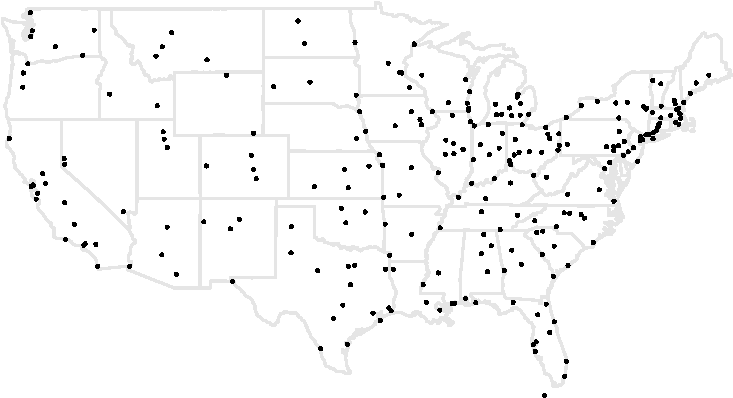
\includegraphics[keepaspectratio]{march-2025-draft_files/figure-pdf/fig-map-1.pdf}}

}

\caption{\label{fig-map}257 American cites; our task is to find the
shortest path that goes through all of them.}

\end{figure}%

The task is to find the shortest path through those 257
cities.\footnote{The 257 cities are the cities in the lower 48 states
  from the 312 cities in North America that John Burkardt
  (\citeproc{ref-Burkhart2011}{2011}) mapped in his dataset USCA312.}

All of the decision theories the critic described in
Section~\ref{sec-two}, and as far as I know every competitor to them in
the philosophical literature, say the thing to do here is to draw
whichever of the 256! possible paths is shortest. That is not
particularly helpful advice. Unless you know a lot about problems like
this, you can't draw the shortest path through the map. More precisely,
you can't draw it as such. You can't draw it in the way that you can't
enter the correct code on a locked phone
(\citeproc{ref-MandelkernEtAl2017}{Mandelkern, Schultheis, and Boylan
2017}).

One of the striking things about this puzzle is that it turns out there
are some helpful things that can be said. One helpful bit of advice to
someone trying to solve a problem like this is to use a Farthest
Insertion Algorithm.\footnote{To implement both this algorithm and the
  optimisation I'll mention below, I've used the TSP package by Michael
  Hashler and Kurt Hornik (\citeproc{ref-HashlerHornik2007}{2007}). The
  description of the two steps owes a lot to their summaries in the
  package documentation.} Insertion algorithms say to start with a
random city, then add cities to the path one at a time, at each time
finding the point to insert the city into the existing path that adds
the least distance. The Farthest Insertion Algorithm says that the city
added at each stage is the one farthest from the existing path.
Insertion algorithms in general produce pretty good paths in a very
short amount of time - at least on normal computers. And the Farthest
Insertion Algorithm is, most of the time, the best Insertion Algorithm
to use. Figure~\ref{fig-farthest} shows the result of one output of this
algorithm.\footnote{The algorithm is silent on which city you start
  with, and usually chooses this randomly.}

\begin{figure}

\centering{

\pandocbounded{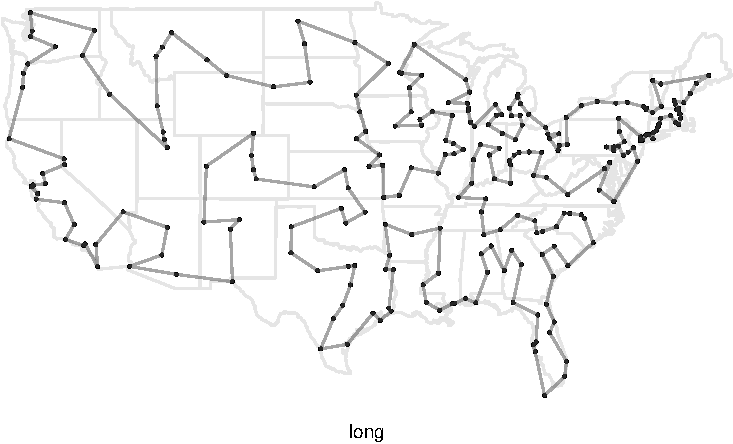
\includegraphics[keepaspectratio]{march-2025-draft_files/figure-pdf/fig-farthest-1.pdf}}

}

\caption{\label{fig-farthest}An output of the Farthest Insertion
Algorithm, with a length of 21075 miles.}

\end{figure}%

The path in Figure~\ref{fig-farthest} is not bad, but with only a bit of
extra computational work, one can do better. A fairly simple
optimisation algorithm takes a map as input, and then deletes pairs of
edges at a time, and finds the shortest path of all possible paths with
all but those two edges. The process continues until no improvements can
be made by deleting two edges at a time, at which point you've found a
somewhat resilient local minimum. Figure~\ref{fig-two-opt} is the output
from applying this strategy to the path in Figure~\ref{fig-farthest}.

\begin{figure}

\centering{

\pandocbounded{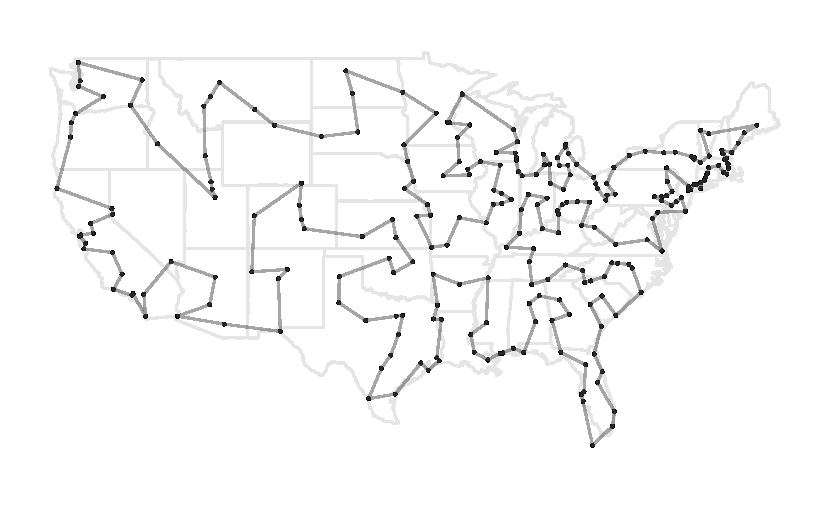
\includegraphics[keepaspectratio]{march-2025-draft_files/figure-pdf/fig-two-opt-1.pdf}}

}

\caption{\label{fig-two-opt}The output of an optimisation process, which
reduced the path length to 20891 miles.}

\end{figure}%

This optimisation tends to produce paths that look a lot like the
original, but are somewhat shorter. For most practical purposes, the
best advice you could give someone faced with a problem like this is to
use a Farthest Insertion Algorithm, then optimise it in this way. Or, if
they have a bit more time, they could do this a dozen or so times, and
see if different starting cities led to slightly shorter paths.

While this is good advice, and indeed it's what most people should do,
it's not typically what is optimal to do. For that reason, it's not what
our nine decision theories would say to do. If one had unlimited and
free computing power available, hacks like these would be pointless. One
would simply look at all the possible paths, and see which was shortest.
I do not have free, unlimited computing power, so I didn't do this.
Using some black box algorithms I did not particularly understand, I was
able to find a shorter path, however. It took some time, both of mine
and my computer's, and for most purposes it would not have been worth
the hassle of finding it. Still, just to show it exists, I've plotted it
as Figure~\ref{fig-best}.

\begin{figure}

\centering{

\pandocbounded{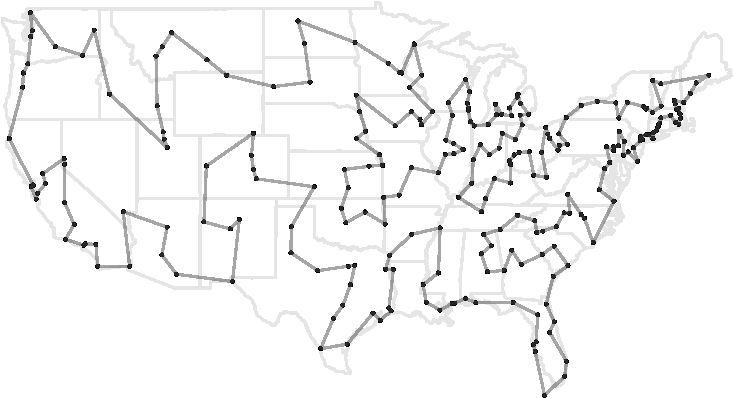
\includegraphics[keepaspectratio]{march-2025-draft_files/figure-pdf/fig-best-1.pdf}}

}

\caption{\label{fig-best}The shortest path I could find, with a distance
of 20301 miles.}

\end{figure}%

I'm not sure if Figure~\ref{fig-best} is as short as possible, but I
couldn't find a shorter one. Still, for many purposes it wouldn't have
been worth the trouble it took to find this map.

\subsection{The Two Cases}\label{the-two-cases}

Table~\ref{tbl-examples} summarises the examples from the last two
sections.

\begin{longtable}[]{@{}lcc@{}}
\caption{How three approaches to decision theory handle the two
cases}\label{tbl-examples}\tabularnewline
\toprule\noalign{}
& Betting & Salesman \\
\midrule\noalign{}
\endfirsthead
\toprule\noalign{}
& Betting & Salesman \\
\midrule\noalign{}
\endhead
\bottomrule\noalign{}
\endlastfoot
Best outcome & Bet on winner & Shortest path \\
Decision theory & Pass & Shortest path \\
Best advice & Pass & Learn algorithms \\
\end{longtable}

The first row says which action would produce the best outcome in the
two cases. The third row says what advice one ought give someone who had
to choose in the two cases. And the middle row says what all the
decision theories say about the two cases. Notably, it agrees with
neither the first nor third row. Decision theory is neither in the
business of saying what will produce the best result, nor with giving
the most useful advice. So what is it doing?

\phantomsection\label{refs}
\begin{CSLReferences}{1}{0}
\bibitem[\citeproctext]{ref-Ahmed2014}
Ahmed, Arif. 2014. \emph{Evidence, Decision and Causality}. Cambridge:
{C}ambridge {U}niversity {P}ress.

\bibitem[\citeproctext]{ref-Akerlof1970}
Akerlof, George. 1970. {``The Market for "Lemons": Quality Uncertainty
and the Market Mechanism.''} \emph{Quarterly Journal of Economics} 84
(3): 488--500. doi:
\href{https://doi.org/10.2307/1879431}{10.2307/1879431}.

\bibitem[\citeproctext]{ref-Arntzenius2008}
Arntzenius, Frank. 2008. {``No Regrets; or, Edith Piaf Revamps Decision
Theory.''} \emph{Erkenntnis} 68 (2): 277--97. doi:
\href{https://doi.org/10.1007/s10670-007-9084-8}{10.1007/s10670-007-9084-8}.

\bibitem[\citeproctext]{ref-Barnett2022}
Barnett, David James. 2022. {``Graded Ratifiability.''} \emph{Journal of
Philosophy} 119 (2): 57--88. doi:
\href{https://doi.org/10.5840/jphil202211925}{10.5840/jphil202211925}.

\bibitem[\citeproctext]{ref-BuchakRisk}
Buchak, Lara. 2013. \emph{Risk and Rationality}. Oxford: Oxford
University Press.

\bibitem[\citeproctext]{ref-Burkhart2011}
Burkardt, John. 2011. {``Cities.''}
\url{https://people.sc.fsu.edu/~jburkardt/datasets/cities/cities.html}.

\bibitem[\citeproctext]{ref-Friedman2020}
Friedman, Jane. 2020. {``The Epistemic and the Zetetic.''}
\emph{Philosophical Review} 129 (4): 501--36. doi:
\href{https://doi.org/10.1215/00318108-8540918}{10.1215/00318108-8540918}.

\bibitem[\citeproctext]{ref-Fuscond}
Fusco, Melissa. n.d. {``Absolution of a Causal Decision Theorist.''}
\emph{No{û}s}. doi:
\href{https://doi.org/10.1111/nous.12459}{10.1111/nous.12459}. Early
view.

\bibitem[\citeproctext]{ref-Gallow2020}
Gallow, J. Dmitri. 2020. {``The Causal Decision Theorist's Guide to
Managing the News.''} \emph{The Journal of Philosophy} 117 (3): 117--49.
doi:
\href{https://doi.org/10.5840/jphil202011739}{10.5840/jphil202011739}.

\bibitem[\citeproctext]{ref-Gustafsson2011}
Gustafsson, Johan E. 2011. {``A Note in Defence of Ratificationism.''}
\emph{Erkenntnis} 75 (1): 147--50. doi:
\href{https://doi.org/10.1007/s10670-010-9267-6}{10.1007/s10670-010-9267-6}.

\bibitem[\citeproctext]{ref-HashlerHornik2007}
Hahsler, Michael, and Kurt Hornik. 2007. {``TSP---Infrastructure for the
Traveling Salesperson Problem.''} \emph{Journal of Statistical Software}
23 (2): 1--21. doi:
\href{https://doi.org/10.18637/jss.v023.i02}{10.18637/jss.v023.i02}.

\bibitem[\citeproctext]{ref-Harper1986}
Harper, William. 1986. {``Mixed Strategies and Ratifiability in Causal
Decision Theory.''} \emph{Erkenntnis} 24 (1): 25--36. doi:
\href{https://doi.org/10.1007/BF00183199}{10.1007/BF00183199}.

\bibitem[\citeproctext]{ref-Joyce1999}
Joyce, James M. 1999. \emph{The Foundations of Causal Decision Theory}.
Cambridge: Cambridge University Press.

\bibitem[\citeproctext]{ref-LevinsteinSoares2020}
Levinstein, Benjamin Anders, and Nate Soares. 2020. {``Cheating Death in
Damascus.''} \emph{Journal of Philosophy} 117 (5): 237--66. doi:
\href{https://doi.org/10.5840/jphil2020117516}{10.5840/jphil2020117516}.

\bibitem[\citeproctext]{ref-Lewis1994b}
Lewis, David. 1994. {``Reduction of Mind.''} In \emph{A Companion to the
Philosophy of Mind}, edited by Samuel Guttenplan, 412--31. Oxford:
Blackwell. doi:
\href{https://doi.org/10.1017/CBO9780511625343.019}{10.1017/CBO9780511625343.019}.
Reprinted in his \emph{Papers in Metaphysics and Epistemology}, 1999,
291-324, Cambridge: Cambridge University Press. References to reprint.

\bibitem[\citeproctext]{ref-Lewis-Gorman-10071979}
---------. (1989) 2020. {``Letter to Jonathan Gorman, 19 April 1989.''}
In \emph{Philosophical Letters of David {K}. Lewis}, edited by Helen
Beebee and A. R. J. Fisher, 1:472--73. Oxford: Oxford University Press.

\bibitem[\citeproctext]{ref-MandelkernEtAl2017}
Mandelkern, Matthew, Ginger Schultheis, and David Boylan. 2017.
{``Agentive Modals.''} \emph{Philosophical Review} 126 (3): 301--43.
doi:
\href{https://doi.org/10.1215/00318108-3878483}{10.1215/00318108-3878483}.

\bibitem[\citeproctext]{ref-Markovits2014}
Markovits, Julia. 2014. \emph{Moral Reason}. Oxford: Oxford University
Press.

\bibitem[\citeproctext]{ref-Podgorski2022}
Podgorski, Aberlard. 2022. {``Tournament Decision Theory.''}
\emph{No{û}s} 56 (1): 176--203. doi:
\href{https://doi.org/10.1111/nous.12353}{10.1111/nous.12353}.

\bibitem[\citeproctext]{ref-Robinson1949}
Robinson, Julia. 1949. {``On the Hamiltonian Game (a Traveling Salesman
Problem).''} Santa Monica, CA: The RAND Corporation.

\bibitem[\citeproctext]{ref-Schelling1971}
Schelling, Thomas C. 1971. \emph{The Journal of Mathematical Sociology}
1 (2): 143--86. doi:
\href{https://doi.org/10.1080/0022250X.1971.9989794}{10.1080/0022250X.1971.9989794}.

\bibitem[\citeproctext]{ref-Schrijver2005}
Schrijver, Alexander. 2005. {``On the History of Combinatorial
Optimization (till 1960).''} \emph{Handbooks in Operations Research and
Management Science} 12: 1--68. doi:
\href{https://doi.org/10.1016/S0927-0507(05)12001-5}{10.1016/S0927-0507(05)12001-5}.

\bibitem[\citeproctext]{ref-Spencer2023}
Spencer, Jack. 2023. {``Can It Be Irrational to Knowingly Choose the
Best?''} \emph{Australasian Journal of Philosophy} 101 (1): 128--39.
doi:
\href{https://doi.org/10.1080/00048402.2021.1958880}{10.1080/00048402.2021.1958880}.

\bibitem[\citeproctext]{ref-wiki-salesman}
Travelling salesman problem. 2024. {``Travelling Salesman Problem---
{W}ikipedia{,} the Free Encyclopedia.''}
\url{https://en.wikipedia.org/w/index.php?title=Travelling_salesman_problem&oldid=1209291065}.
{[}Online; accessed 27-February-2024{]}.

\bibitem[\citeproctext]{ref-Vredenburgh2024}
Vredenburgh, Kate. 2024. {``Causal Explanation and Revealed
Preferences.''} \emph{Philosophy of Science} 91 (2): 269--87. doi:
\href{https://doi.org/10.1017/psa.2023.112}{10.1017/psa.2023.112}.

\bibitem[\citeproctext]{ref-Wedgwood2013a}
Wedgwood, Ralph. 2013. {``Gandalf's Solution to the Newcomb Problem.''}
\emph{Synthese} 190 (14): 2643--75. doi:
\href{https://doi.org/10.1007/s11229-011-9900-1}{10.1007/s11229-011-9900-1}.

\bibitem[\citeproctext]{ref-Weisberg2007}
Weisberg, Michael. 2007. {``Three Kinds of Idealization.''} \emph{The
Journal of Philosophy} 104 (12): 639--59. doi:
\href{https://doi.org/10.5840/jphil20071041240}{10.5840/jphil20071041240}.

\bibitem[\citeproctext]{ref-MWeisberg2013}
---------. 2013. \emph{Simulation and Similarity: Using Models to
Understand the World}. Oxford: Oxford University Press.

\end{CSLReferences}



\noindent Unpublished. Posted online in 2025.


\end{document}
